\newcommand*\mycirc[1]{%
   \begin{tikzpicture}
     \node[draw,circle,inner sep=1pt,color=blue ] {#1};
   \end{tikzpicture}}
Adding slack variables to the left side of \eqref{eq:solutions/4/38/eq:2} and \eqref{eq:solutions/4/38/eq:3},we get
\begin{align}
    Z-4x-y=0\\
    x+y+s_1=50\\
    3x+y+s_2=90
\end{align}
Forming simplex tableau,
\begin{align}
    \myvec{x & y & s_1 & s_2 & b \\\hline
    1 & 1 & 1 & 0 & 50 \\
    \mycirc{3} & 1 & 0 & 1 & 90 \\\hline
    -4 & -1 & 0 & 0 & 0}
\end{align}
-4 is the smallest entry in the bottom row. Therefore, we determine that x is the starting variable.\\
Also, the smallest positive ratio is 30, therefore, we chose $s_2$ as the departing variable.\\
Hence, keeping the pivot element as 3, we perform  Gauss Jordan elimination,
\begin{align}
    \myvec{x & y &s_1 & s_2 & b\\
    1 & 1 & 1 & 0 & 50\\
    1 & \frac{1}{3} & 0 & \frac{1}{3} & 30\\\hline
    -4 & -1 & 0 & 0 & 0}\\
    \myvec{x & y &s_1 & s_2 & b\\
    0 & \frac{2}{3} & 1 & \frac{-1}{3} & 20\\
    1 & \frac{1}{3} & 0 & \frac{1}{3} & 30\\\hline
    0 & \frac{1}{3} & 0 & \frac{4}{3} & 120}
\end{align}
Note that x has replaced in the basis column $s_2$ and the improved solution
\begin{align}
    (x,y,s_1,s_2)=(30,0,20,0)
\end{align}
maximizes Z to value
\begin{align}
    Z=4(30)+3(0)\\
    Z=120
\end{align}
The given problem can be expressed in the form of matrix inequality as:
\begin{align}
    \max_{\{x\}}\vec{c}^T\Vec{x}\\
    s.t \quad \Vec{A}\vec{x}\leq \vec{b}\\
    \Vec{x} \geq 0\\
\end{align}
where
\begin{align}
    \Vec{c}=\myvec{4\\1}\\
    \Vec{A}=\myvec{1 & 1\\3 & 1}\\
    \Vec{b}=\myvec{50\\90}
\end{align}
can be solved using Python. The plot obtained from python is attached below:
\begin{figure}[!ht]
\centering
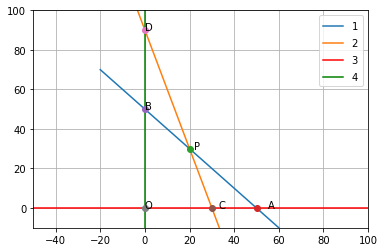
\includegraphics[width=\columnwidth]{./solutions/4/38/LPP.png}
\caption{Plot obtained from python code}
\label{eq:solutions/4/38/Fig:1}
\end{figure}
